% Drawing 161-6/01-8 -- folder 161-6, batch 01, archive page 17 (PDF page 18).
% Transcription: plus à droite, à l'encre, deux cercles tangents : celui de gauche porte deux axes, l'un à peu près horizontal, l'autre vertical, et un rayon épais vers le haut à gauche ; celui de droite, plus grand et resté ouvert en haut à droite, un angle épais dont la pointe est tournée vers le bas.
% Kind: two tangent circles, one with axes, one with an angle. Method 2 (schematic redraw from the facsimile). Status: ok.
% Notes: Two circles fitted to his outlines, touching at one point. Left circle: the two axes through one centre, the heavy radius to the upper left, the thin stroke hanging from its outer end, the dot near the left end of the horizontal axis. Right circle: open at the upper right as on the page; the heavy angle (two strokes meeting at their lower end) and the short tick under it. Left out: the doubling of the outlines near the point of contact, a small loop on the lower outline of the right circle, two small ink marks near the centre of the left circle, and the faint pencil strokes that run into the left circle from the left. Redrawn 2026-11-12 (issue 128): to check again.
% Coordinates: 1 unit = 1 mm = 1/100 of the crop width; labels turned as on the page (leaf written across (the writing runs up the scanned page); drawn as the scan shows it, labels turned as on the page) (bbox in page fractions: [0.38, 0.099, 0.59, 0.198]).
% Redrawn by Claude (claude-fable-5-2), issue #128, 2026-11-12; not checked by a human; not compiled (no TeX in the session).
% Rights: reproduces part of the work -- behind RENDER_TRANSCRIPTS, never published by itself.
\documentclass[tikz,border=3pt]{standalone}
\usepackage{amsmath,amssymb}
\usetikzlibrary{patterns,arrows.meta}
\tikzset{pencil/.style={black!45}, struck/.style={black!35}, mpt/.style={circle,draw,inner sep=1.3pt}, pt/.style={circle,fill,inner sep=0.9pt}, opt/.style={circle,draw,fill=white,inner sep=1.1pt}}
\begin{document}
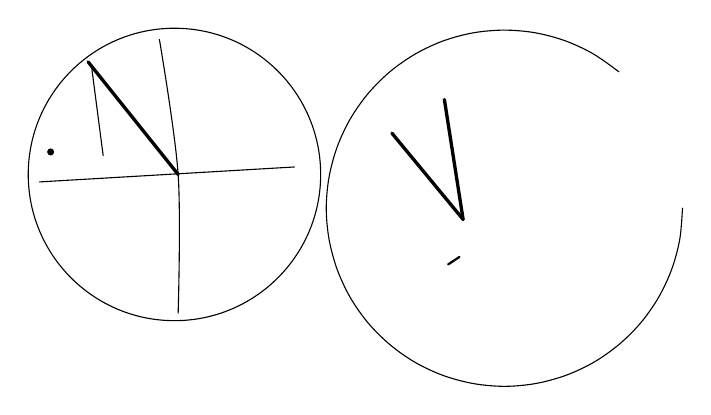
\begin{tikzpicture}[x=1mm,y=1mm,line cap=round,line join=round,font=\small]
\draw (30.48,-28.58) circle[radius=18.57];
\draw (13.33,-29.53) -- (45.71,-27.63);
\draw plot[smooth, tension=0.55] coordinates {(28.57,-11.44) (30.95,-28.58) (30.95,-46.2)};
\draw[very thick] (19.52,-14.29) -- (30.95,-28.58);
\draw (20,-15.25) -- (21.43,-26.2);
\node[pt] at (14.76,-25.72) {};
\draw plot[smooth, tension=0.55] coordinates {(86.92,-15.54) (83.69,-13.28) (80.12,-11.61) (76.31,-10.59) (72.38,-10.25) (68.45,-10.59) (64.64,-11.61) (61.07,-13.28) (57.84,-15.54) (55.05,-18.33) (52.79,-21.56) (51.13,-25.13) (50.11,-28.94) (49.76,-32.87) (50.11,-36.79) (51.13,-40.6) (52.79,-44.18) (55.05,-47.41) (57.84,-50.19) (61.07,-52.46) (64.64,-54.12) (68.45,-55.14) (72.38,-55.49) (76.31,-55.14) (80.12,-54.12) (83.69,-52.46) (86.92,-50.19) (89.71,-47.41) (91.97,-44.18) (93.64,-40.6) (94.66,-36.79) (95,-32.87)};
\draw[very thick] (64.76,-19.06) -- (67.14,-34.29);
\draw[very thick] (58.1,-23.34) -- (67.14,-34.29);
\draw[thick] (65.24,-40.01) -- (66.67,-39.06);
\end{tikzpicture}
\end{document}
